



\chapter{Arithmétique}



\section{Rappels : nombres entiers}

\begin{Définition}
L'ensemble des nombres {\bf{entiers naturels}}, noté $\N$ , est l'ensemble des nombres entiers positifs ou
nul.\\
L'ensemble des nombres {\bf{entiers relatifs}}, noté $\Z$ , est l'ensemble des nombres entiers positifs,
négatifs ou nul.
\end{Définition}

\begin{minipage}[c]{0.5\linewidth}

\begin{Remarque}
Tout nombre entier naturel est un entier relatif. \\On a $\N\subset\Z$.
\end{Remarque}
\end{minipage} \hfill
\begin{minipage}[c]{0.45\linewidth}
\begin{center} \begin{tikzpicture}[scale=.75] 

\def\Z{ (-0.4,0.6) rectangle (4,3) };
\def\N{ (-0.2,0.8) rectangle (2,2) };




\begin{scope}
\clip \Z ;
\fill[Couleur6!10] \Z ;
\end{scope}



\begin{scope}
\clip \Z ;
\fill[Couleur1!30] \N;
\end{scope}


\draw[Couleur6!75!black] \Z ;
\draw[Couleur1] \N ;


\draw[Couleur6!75!black] (3.7,2.7) node{$\mathbb{Z}$} ; 
\draw[Couleur1] (1.7,1.7) node{$\mathbb{N}$} ; 


\draw (0.4,1.6) node{$5$} ; 
\draw (1.3,1.1) node{$2586$} ; 
\draw (3,1.2) node{$-365$} ; 
\draw (1.1,2.5) node{$-24$} ; 
\draw (2.8,2.3) node{$-7$} ; 

\end{tikzpicture} 
\end{center}
\end{minipage}





\section{Multiples et diviseurs}
\begin{Définition}
Soient $a$ et $b$ deux entiers. \\On dit que $a$ est un {\bf{multiple}} de $b$ s'il existe un entier $k$
tel que $a = k\times b$. On dit alors que $b$ est un {\bf{diviseur}} de $a$.
\end{Définition}
\begin{Exemple}
\leavevmode\vspace{-\baselineskip}
\begin{itemize}[label=\textcolor{Couleur8}{$\bullet$}]
\item $15$ est un multiple de $3$, car $15 = 5 \times 3$.
\item $10$ est un diviseur de $80$, car $80 = 8 \times 10$. 
\item Par contre, $13$ n'est pas un multiple de $3$ car il n'existe pas d'entier $k$ tel que $13 = k \times 3$.
\end{itemize}
\end{Exemple}
\begin{Propriété}
Soient $a$, $n$ et $m$ trois entiers relatifs.
\\Si $n$ et $m$ sont deux multiples de $a$, alors leur somme $(n+m)$, leur différence $(n-m)$ et leur
produit $n\times m$ sont aussi des multiples de $a$.
\end{Propriété}

\begin{proof}
Pour la somme : \\$n$ et $m$ sont des multiples de $a$. Donc il existe $k$ et $q$ des entiers relatifs tel que $m=k\times a$ et $n=q\times a$. \\Alors $m+n=k\times a+q\times a=(k+q)\times a$. Or, $k+q\in \Z$, donc $m+n$ est un multiple de $a$.
\end{proof}

\begin{Exemple}
$54$ et $90$ sont des multiples de $9$. Donc $54+90=144$ est un multiple de $9$. En effet, $144=16\times 9$. 
\end{Exemple}



\paragraph{Retour sur la propriété : $\dfrac{1}{3}$ n'est pas décimal.}

\begin{proof}
Démontrons que le nombre rationnel $\dfrac{1}{3}$ n'est pas décimal.\\
On va effectuer une démonstration par l'absurde en supposant que $\dfrac{1}{3}$ est décimal.\\
Si notre démonstration aboutit à une absurdité, cela prouvera que notre hypothèse de départ est fausse. \\

\noindent Supposons donc que $\dfrac{1}{3}$ est décimal. 
Alors il s'écrit sous la forme  $\dfrac{1}{3}=\dfrac{a}{10^p}$ avec $a$ entier et $p$ entier naturel. \\

\noindent Donc $10^p = 3a$ et donc $10^p$ est divisible par $3$.
Un nombre est divisible par $3$ lorsque la somme de ses chiffres est divisible par $3$.
Or, ceci est impossible car la somme des chiffres de $10^p$ est $1$, et $1$ n'est pas divisible par $3$.\\
Donc l'hypothèse posée au départ est fausse et donc $\dfrac{1}{3}$ n'est pas décimal
\end{proof}

\newpage

\section{Nombres pairs et impairs}
\begin{Définition}
On considère un entier relatif $n$ .
On dit que $n$ est {\bf{pair s'il est divisible par}} $2$, alors il existe $k\in \Z$ tel que $n=2\times k$ .
Sinon on dit que $n$ est {\bf{impair}}, alors il existe $k\in \Z$ tel que $n=2\times k +1$
\end{Définition}
\begin{Exemple}
\leavevmode\vspace{-\baselineskip}
\begin{multicols}{2}
\begin{itemize}[label=\textcolor{Couleur8}{$\bullet$}]
\item $18$ est pair car $18=2\times 9$.
\item $0$ est pair car $0=2\times 0$.
\item $17$ est impair car $17=2\times 8+1$.
\item $1$ est impair car $1=2\times 0 +1$.
\end{itemize}
\end{multicols}
\end{Exemple}

\begin{Propriété}
La somme (ou la différence) de deux nombres pairs est un nombre pair.\\
La somme (ou la différence) de deux nombres impairs est un nombre pair.
\end{Propriété}

\begin{Exemple}
$46$ et $28$ sont des nombres pairs et $46+28=64$ et $46-28=18$ sont aussi des nombres pairs.\\
$15$ et $37$ sont des nombres impairs et $37+15=52$ et $15-37=-22$ sont des nombres pairs.
\end{Exemple}

\begin{Propriété}
Soit $n\in \Z$. \\
Si $n$ est pair, alors le carré $n^2$ est pair.\\
Si $n$ est impair, alors le carré $n^2$ est impair.
\end{Propriété}

\begin{proof}
Pour le carré d'un nombre impair :\\
$n$ est un nompre impair, donc il existe $k\in \Z$ tel que $n=2k+1$. \\Alors $n^2=(2k+1)^2=(2k)^2+2\times 2k\times 1 +1^2=4k^2+4k+1=2\times (2k^2+2k)+1=2K+1$, avec $K=2k^2+2k \in \Z$. \\Donc $n^2$ est impair.
\end{proof}

\begin{Exemple}
\leavevmode\vspace{-\baselineskip}
\begin{itemize}[label=\textcolor{Couleur8}{$\bullet$}]
\item $11$ est impair et $11^2=121$ est impair.
\item $12$ est pair et $12^2=144$ est pair.
\end{itemize}
\end{Exemple}



\section{Nombres premiers}

\begin{Définition}
Un nombre entier naturel est premier s'il possède que deux diviseurs positifs distincts qui sont $1$ et lui-même.
\end{Définition}

\begin{Exemple}
\leavevmode\vspace{-\baselineskip}
\begin{itemize}[label=\textcolor{Couleur8}{$\bullet$}]
\item $2,3,5,7,11,13,17,19,23,...$ sont des nombres premiers, cette liste est infinie.
\item $1$ n'est pas premier car son seul diviseur positif est $1$.
\end{itemize}
\end{Exemple}

\begin{Définition}
On dit que deux nombres sont premiers entre eux lorsque leur seul
diviseur commun est $1$.
\end{Définition}

\newpage

\begin{Propriété}
Tout nombre supérieur ou égal à $2$ peut se décomposer en produits de facteurs premiers. Cette décomposition est unique à l'ordre des facteurs près.
\end{Propriété}

\begin{Exemple}
$300=2\times 2\times 3\times 5\times 5$ et $77=7\times 11$. \\Ainsi, le seul diviseur commun à $300$ et $77$ est $1$ donc $300$ et $77$ sont premiers entre eux.
\end{Exemple}

\begin{Propriété}
On dit qu'une fraction est irréductible, lorsque son numérateur et son dénominateur sont premiers entre eux.
\end{Propriété}

\begin{Méthode}Rendre une fraction irréductible.
Rendre irréductible la fraction $\dfrac{210}{196}$.\\
Décomposons d'abord le numérateur et le dénominateur en produits de facteurs premiers.\\

\begin{minipage}[c]{0.3\linewidth}
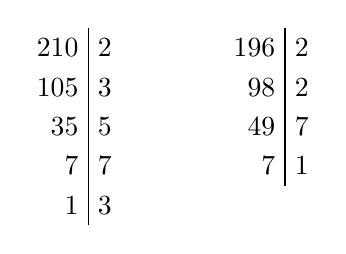
\begin{tikzpicture}
[x=0.5cm,y=0.5cm]
\draw (0,0.5)--(0,-4.5) ; 
\draw (0,0) node[left]{$210$};
\draw (0,0) node[right]{$2$};
\draw (0,-1) node[left]{$105$};
\draw (0,-1) node[right]{$3$};
\draw (0,-2) node[left]{$35$};
\draw (0,-2) node[right]{$5$};
\draw (0,-3) node[left]{$7$};
\draw (0,-3) node[right]{$7$};
\draw (0,-4) node[left]{$1$};
\draw (0,-4) node[right]{$3$};
\draw (5,0.5)--(5,-3.5) ; 
\draw (5,0) node[left]{$196$};
\draw (5,0) node[right]{$2$};
\draw (5,-1) node[left]{$98$};
\draw (5,-1) node[right]{$2$};
\draw (5,-2) node[left]{$49$};
\draw (5,-2) node[right]{$7$};
\draw (5,-3) node[left]{$7$};
\draw (5,-3) node[right]{$1$};
\end{tikzpicture}
\end{minipage} \hfill
\begin{minipage}[c]{0.6\linewidth}
Ainsi, $210=2\times 3\times 5 \times 7$ et $196=2\times 2\times 7\times 7$. \\
Donc $\dfrac{210}{196}=\dfrac{{\color{orange}{2}}\times 3\times 5 \times {\color{orange}{7}}}{{\color{orange}{2}}\times 2\times {\color{orange}{7}}\times 7}=\dfrac{3\times 5}{2\times 7}=\dfrac{15}{14}$. \\
$15$ et $14$ sont premiers entre eux donc, $\dfrac{15}{14}$ est la fraction irréductible de $\dfrac{210}{196}$.
\end{minipage}

\end{Méthode}

\paragraph{Retour sur la propriété : $\sqrt{2}$ est un nombre irrationnel.}
\begin{proof}
On va effectuer une démonstration par l'absurde en supposant que $\sqrt{2}$ est rationnel. \\Si notre démonstration aboutit à une absurdité, cela prouvera que notre hypothèse de départ est fausse.
Supposons donc que $\sqrt{2}$ est un rationnel.
Il s'écrit alors $\sqrt{2}=\dfrac{p}{q}$ avec $p$ et $q$ entiers naturels premiers entre eux, $b$ non nul.\\
Ainsi, $\dfrac{p^2}{q^2}=\left(\sqrt{2}\right)^2=2$ soit $p^2=2q^2$.
On en déduit que $p^2$ est pair, ce qui entraîne que $p$ est pair.
\\En effet, si $p$ était impair, alors $p^2$ serait impair.
Puisque $p$ est pair, il existe un entier naturel $k$ tel que $p = 2k$. \\Comme, $p^2=2q^2$, on a $(2k)^2=2q^2$, soit $4k^2=2q^2$, qui se simplifie en $q^2=2k^2$. On en déduit que $q^2$ est pair, ce qui entraîne que $q$ est pair. Or, $p$ et $q$ sont premiers entre eux, donc ils ne peuvent pas être pairs simultanément. \\On aboutit à une absurdité. Donc, $\sqrt{2}$ n'est pas un rationnel. Finalement, $\sqrt{2}$ est un irrationnel.
\end{proof}

\bigskip

\newpage

\section*{Exercices - Arithmétique}
\addcontentsline{toc}{section}{Exercices}
{\setlength{\columnseprule}{0pt}
\setcounter{NumEx}{1}

\arrayrulecolor{Couleur6}

\renewcommand{\arraystretch}{1.3}  % augmente la hauteur de 50%

\subsection*{Multiples et diviseurs}

% @see : https://coopmaths.fr/alea?uuid=7cf48&id=2N20-1&n=6&d=10&s=2-3&s2=8&s3=12&s4=3&alea=xOLc&cd=1&cols=1
\begin{Exercice}
\leavevmode\vspace{-\baselineskip}

\begin{enumerate}[itemsep=1em]
	\item \begin{minipage}[t]{\linewidth}Écrire la liste de tous les diviseurs de 184.\end{minipage}
	\item \begin{minipage}[t]{\linewidth}Écrire la liste de tous les diviseurs de 927.\end{minipage}
	\item \begin{minipage}[t]{\linewidth}Compléter le tableau suivant et faire la liste de tous les diviseurs de 70.$\medskip$\\$\begin{array}{|c|c|c|}
\hline
\text{Facteur n°1} & \text{Facteur n°2} & \text{Produit donnant } 70 \\
\hline
\ldots & 70& \ldots \\
\hline
\ldots & \ldots& 70 \\
\hline
5 & \ldots& \ldots \\
\hline
7 & 10& 70 \\
\hline
\end{array}
$\\\end{minipage}
	\item \begin{minipage}[t]{\linewidth}Écrire la liste de tous les diviseurs de 154.\end{minipage}
	\item \begin{minipage}[t]{\linewidth}Compléter le tableau suivant et faire la liste de tous les diviseurs de 12.$\medskip$\\$\begin{array}{|c|c|c|}
\hline
\text{Facteur n°1} & \text{Facteur n°2} & \text{Produit donnant } 12 \\
\hline
\ldots & \ldots& 12 \\
\hline
\ldots & \ldots& \ldots \\
\hline
\ldots & 4& 12 \\
\hline
\end{array}
$\\\end{minipage}
	\item \begin{minipage}[t]{\linewidth}Compléter le tableau suivant et faire la liste de tous les diviseurs de 30.$\medskip$\\$\begin{array}{|c|c|c|}
\hline
\text{Facteur n°1} & \text{Facteur n°2} & \text{Produit donnant } 30 \\
\hline
\ldots & 30& \ldots \\
\hline
\ldots & \ldots& 30 \\
\hline
3 & 10& 30 \\
\hline
5 & \ldots& \ldots \\
\hline
\end{array}
$\\\end{minipage}
\end{enumerate}


\end{Exercice}

% @see : https://coopmaths.fr/alea?uuid=d5a6d&id=2N20-2&n=8&d=10&s=true&alea=strE&cd=1&cols=1
\begin{Exercice}
Compléter le tableau en mettant oui ou non dans chaque case.\\


 \begin{minipage}[t]{\linewidth}
\begin{center}


$\begin{array}{|l|c|c|c|c|c|c|}
\hline
\text{... est divisible} & \text{par }2 & \text{par }3 & \text{par }4 & \text{par }5 & \text{par }9 & \text{par }10\\
\hline
31\,937 & & & & & & \\
\hline
346\,326 & & & & & & \\
\hline
207\,399 & & & & & & \\
\hline
809\,442 & & & & & & \\
\hline
86\,078 & & & & & & \\
\hline
5\,659\,110 & & & & & & \\
\hline
727\,310 & & & & & & \\
\hline
501\,759 & & & & & & \\
\hline
\end{array}$



\end{center}
\end{minipage}

\end{Exercice}

\newpage

% @see : https://coopmaths.fr/alea?uuid=098db&id=2N20-3&n=5&d=10&s=3&s2=8&s3=15&alea=K5h3&cd=0&cols=1
\begin{Exercice}
\leavevmode\vspace{-\baselineskip}

\begin{enumerate}[itemsep=2em]
	\item \begin{minipage}[t]{\linewidth}Quel est le plus grand reste possible dans une division euclidienne par 62 ?\end{minipage}
	\item \begin{minipage}[t]{\linewidth}On a \numprint{32050}=37$\times$866 $+$ 8\\Écrire le quotient et le reste de la division euclidienne de \numprint{32050} par 37.\end{minipage}
	\item \begin{minipage}[t]{\linewidth}Les trois divisions euclidiennes suivantes sont exactes : \\\numprint{5653} = \numprint{5653}$\times$1 $+$ 0\\\numprint{5653} = \numprint{5652}$\times$1 $+$ 1\\\numprint{5653} = \numprint{5654}$\times$0 $+$ \numprint{5653}\\Sans calculer, dire si les nombres \numprint{5653}; \numprint{5652}; \numprint{5654} sont des diviseurs de \numprint{5653}. Justifier.\end{minipage}
	\item \begin{minipage}[t]{\linewidth}Après avoir testé avec la calculatrice, compléter chaque phrase avec "est un diviseur de" ou "est un multiple de" ou "n'est ni un diviseur, ni un multiple de".\\386 $\ldots\ldots\ldots\ldots$ 757\\427 $\ldots\ldots\ldots\ldots$ \numprint{3416}\\\numprint{2910} $\ldots\ldots\ldots\ldots$ 582\\104 $\ldots\ldots\ldots\ldots$ 624\\680 $\ldots\ldots\ldots\ldots$ 85\\937 $\ldots\ldots\ldots\ldots$ 64\end{minipage}
	\item \begin{minipage}[t]{\linewidth}Écrire la liste de tous les diviseurs de 938.\end{minipage}
\end{enumerate}
\end{Exercice}

\begin{Exercice}
Soit $ a $ et $ b $ deux entiers. Montrer que si $ a $ est un diviseur de $ b $, alors $ a^2 $ est un diviseur de $ b^2 $.
\end{Exercice}

\begin{Exercice}
Soit $ n $ un entier naturel.
On pose $ a = 2n - 7 $ et $ b=n + 1 $.
\begin{enumerate}
\item Calculer $ a - 2b $.
\item Soit $ d $ un diviseur de $ a $ et $ b $. Montrer que $ d $ est un diviseur de $ a - 2b $.
\item Soit $ d $ un entier diviseur de $ a $ et $ b $.
Quelles sont les valeurs possibles de $ d $ ?
\end{enumerate}
\end{Exercice}

\begin{Exercice}
Un facteur discute avec un professeur de mathématiques :
« Quels âges ont vos trois filles ? »\\
« Le produit de leurs âges fait 36, et leur somme est le numéro de la maison d'en face. » répond le papa taquin.\\
Le facteur réfléchit, puis dit « Vous n'oubliez pas quelque chose ? »\\
Ah si, dit le prof, vous avez raison j'ai oublié de préciser que l'ainée est blonde.\\
C'est bon, dit le facteur, je sais leurs âges alors !\\
Quels âges ont les trois filles ?
\end{Exercice}

\newpage

\subsection*{Parité}


% @see : https://coopmaths.fr/alea?uuid=3ec5c&id=2N20-8&n=6&d=10&alea=Qdsw&cd=1&cols=2
\begin{Exercice}
Soit $n$ un entier naturel.
\vspace{-0.5cm}
\begin{multicols}{2}
\begin{enumerate}[itemsep=1em]
	\item \begin{minipage}[t]{\linewidth}Que peut-on dire de la parité de $5n+4$ ?\end{minipage}
	\item \begin{minipage}[t]{\linewidth}Que peut-on dire de la parité de 3$n$ ?\end{minipage}
	\item \begin{minipage}[t]{\linewidth}Que peut-on dire de la parité de $6n^{2}$ ?\end{minipage}
	\item \begin{minipage}[t]{\linewidth}Que peut-on dire de la parité de $5n+6$ ?\end{minipage}
	\item \begin{minipage}[t]{\linewidth}Que peut-on dire de la parité de $3n^{2}$ ?\end{minipage}
	\item \begin{minipage}[t]{\linewidth}Que peut-on dire de la parité de 6$n$ ?\end{minipage}
\end{enumerate}
\end{multicols}
\end{Exercice}


\begin{Exercice}
Montrer que la somme d'un nombre pair et d'un nombre impair est un nombre impair.
\end{Exercice}

\begin{Exercice}
Montrer que la somme de deux nombres pairs est un nombre pair.
\end{Exercice}

\begin{Exercice}
Montrer que le produit de deux nombres pairs est un multiple de 4.
\end{Exercice}

\begin{Exercice}
Montrer que si $ n $ est un entier pair, alors l'entier $  a =n^2 (n + 20) $ est un multiple de 8.
\end{Exercice}



\begin{Exercice}
\leavevmode\vspace{-\baselineskip}
\begin{enumerate}

\item Le produit d'un nombre pair par un nombre impair est-il pair ou impair ?
\item Soit $ n $ un entier naturel. Montrer que $ (n + 1)(n + 2) $ est pair. On pourra d'abord étudier le cas où $ n $ est pair, puis le cas où $ n $ est impair.
\end{enumerate}
\end{Exercice}



\subsection*{Nombres premiers}

% @see : https://coopmaths.fr/alea?uuid=c04cc&id=2N20-4&n=9&d=10&s=1&s2=false&s3=false&alea=PjcF&cd=1&cols=2
\begin{Exercice}
Justifier que les nombres suivants sont premiers ou pas.    
    \begin{multicols}{3}
\begin{enumerate}[itemsep=1em]
	\item \begin{minipage}[t]{\linewidth}561\end{minipage}
	\item \begin{minipage}[t]{\linewidth}108\end{minipage}
	\item \begin{minipage}[t]{\linewidth}670\end{minipage}
	\item \begin{minipage}[t]{\linewidth}53\end{minipage}
	\item \begin{minipage}[t]{\linewidth}321\end{minipage}
	\item \begin{minipage}[t]{\linewidth}760\end{minipage}
	\item \begin{minipage}[t]{\linewidth}360\end{minipage}
	\item \begin{minipage}[t]{\linewidth}41\end{minipage}
	\item \begin{minipage}[t]{\linewidth}261\end{minipage}
\end{enumerate}
\end{multicols}
\end{Exercice}

\newpage

% @see : https://coopmaths.fr/alea?uuid=c14e8&id=2N20-5&n=9&d=10&s=3&s2=true&s3=true&s4=false&alea=vMkA&cd=0&cols=1
\begin{Exercice}
Écrire les nombres suivants sous la forme d'un produit de facteurs premiers.
\begin{multicols}{3}
\begin{enumerate}[itemsep=1em]
	\item \begin{minipage}[t]{\linewidth}$ 72 $\end{minipage}
	\item \begin{minipage}[t]{\linewidth}$ 360\,360 $\end{minipage}
	\item \begin{minipage}[t]{\linewidth}$ 109\,200 $\end{minipage}
	\item \begin{minipage}[t]{\linewidth}$ 304\,920 $\end{minipage}
	\item \begin{minipage}[t]{\linewidth}$ 7\,200 $\end{minipage}
	\item \begin{minipage}[t]{\linewidth}$ 378 $\end{minipage}
	\item \begin{minipage}[t]{\linewidth}$ 35\,280 $\end{minipage}
	\item \begin{minipage}[t]{\linewidth}$ 98\,280 $\end{minipage}
	\item \begin{minipage}[t]{\linewidth}$ 1\,144 $\end{minipage}
\end{enumerate}
\end{multicols}
\end{Exercice}



\renewcommand{\arraystretch}{1.1} 
% @see : https://coopmaths.fr/alea?uuid=74939&id=2N20-6&n=2&d=10&s=true&alea=lV4n&cd=1&cols=1
\begin{Exercice}
Sans la calculatrice, compter/lister les diviseurs d'un entier à partir de sa décomposition en facteurs premiers.

\begin{enumerate}[itemsep=1em]

	\item \begin{minipage}[t]{\linewidth}La décomposition en facteurs premiers de $29\,645$ est : $5\times 7^{2}\times 11^{2}$. \\\textbf {a.}  Compléter le tableau ci-dessous.$\medskip$\\
	\begin{center} 

$\begin{array}{|c|c|c|}
\hline
\times & \phantom{plusLarge}5^{0}\phantom{plusLarge} & \phantom{plusLarge}5^{1}\phantom{plusLarge}\\
\hline
7^{0}\times11^{0} & & \\
\hline
7^{0}\times11^{1} & & \\
\hline
7^{0}\times11^{2} & & \\
\hline
7^{1}\times11^{0} & & \\
\hline
7^{1}\times11^{1} & & \\
\hline
7^{1}\times11^{2} & & \\
\hline
7^{2}\times11^{0} & & \\
\hline
7^{2}\times11^{1} & & \\
\hline
7^{2}\times11^{2} & & \\
\hline
\end{array}$

\end{center}
$\medskip$\\\textbf {b.}  En déduire le nombre de diviseurs de $29\,645$.\\\textbf {c.}  Enfin, dresser la liste des diviseurs de $29\,645$.\\\end{minipage}
	\item \begin{minipage}[t]{\linewidth}La décomposition en facteurs premiers de $13\,013$ est : $7\times 11\times 13^{2}$. \\\textbf {a.}  Compléter le tableau ci-dessous.$\medskip$\\\begin{center}
$\begin{array}{|c|c|c|}
\hline
\times & \phantom{plusLarge}7^{0}\phantom{plusLarge} & \phantom{plusLarge}7^{1}\phantom{plusLarge}\\
\hline
11^{0}\times13^{0} & & \\
\hline
11^{0}\times13^{1} & & \\
\hline
11^{0}\times13^{2} & & \\
\hline
11^{1}\times13^{0} & & \\
\hline
11^{1}\times13^{1} & & \\
\hline
11^{1}\times13^{2} & & \\
\hline
\end{array}$

	\end{center}
$\medskip$\\\textbf {b.}  En déduire le nombre de diviseurs de $13\,013$.\\\textbf {c.}  Enfin, dresser la liste des diviseurs de $13\,013$.\\\end{minipage}
\end{enumerate}
\end{Exercice}
\newpage
% @see : https://coopmaths.fr/alea?uuid=c3c84&id=2N20-7&n=4&d=10&s=true&alea=JLr6&cd=1&cols=1
\begin{Exercice}
\leavevmode\vspace{-\baselineskip}    
\begin{enumerate}[itemsep=2em]
	\item \begin{minipage}[t]{\linewidth}La roue n$^\circ$1 possède $12$ dents et la roue n$^\circ$2 a $30$ dents.\\\textbf {a.}  Écrire la liste des multiples de $12$ et de $30$ jusqu'à trouver un multiple commun.?\\\textbf {b.}  En déduire le nombre de tours de chaque roue avant le retour à leur position initiale.\end{minipage}
	\item \begin{minipage}[t]{\linewidth}La roue n$^\circ$1 possède $76$ dents et la roue n$^\circ$2 a $57$ dents.\\\textbf {a.}  Décomposer $76$ et $57$ en produit de facteurs premiers.?\\\textbf {b.}  En déduire le nombre de tours de chaque roue avant le retour à leur position initiale.\end{minipage}
	\item \begin{minipage}[t]{\linewidth}La roue n$^\circ$2 a maintenant $135$ dents. Déterminer le nombre de dents de la roue n$^\circ$1 qui ferait $9$  tours  pendant que la roue n$^\circ$2 en fait $2$.\end{minipage}
\end{enumerate}
\end{Exercice}



% @see : https://coopmaths.fr/alea?uuid=8c05e&id=3A12-1&n=3&d=10&s=4&alea=W69f&cd=1&cols=1
\begin{Exercice}
\leavevmode\vspace{-\baselineskip}
\begin{enumerate}[itemsep=1em]
	\item \begin{minipage}[t]{\linewidth}Un fleuriste dispose de 165 iris et de 363 roses. \\Il veut, en utilisant toutes ses fleurs, réaliser un maximum de bouquets contenant tous le même nombre d'iris et le même nombre de roses. 

\medskip
\textbf {a.} Quel est le nombre maximal de bouquets ?

\medskip
\textbf {b.} Quel est le nombre d'iris dans chaque bouquet ?

\medskip
\textbf {c.} Quel est le nombre de roses dans chaque bouquet ?

\medskip
\end{minipage}
	\item \begin{minipage}[t]{\linewidth}Un professeur organise une sortie pédagogique au Futuroscope pour ses élèves de 3ème. Il est accompagné de 74 garçons et de 407 filles. \\Il souhaite répartir tous les élèves en réalisant un maximum de groupes contenant tous le même nombre de garçons et le même nombre de filles. 

\medskip
\textbf {a.} Quel est le nombre maximal de groupes ?

\medskip
\textbf {b.} Quel est le nombre de garçons dans chaque groupe ?

\medskip
\textbf {c.} Quel est le nombre de filles dans chaque groupe ?

\medskip
\end{minipage}
	\item \begin{minipage}[t]{\linewidth}Un boulanger dispose de 418 croissants et de 266 brioches. \\Il veut, en utilisant toutes ses viennoiseries, réaliser un maximum de corbeilles contenant toutes le même nombre de croissants et le même nombre de brioches. 

\medskip
\textbf {a.} Quel est le nombre maximal de corbeilles ?

\medskip
\textbf {b.} Quel est le nombre de croissants dans chaque corbeille ?

\medskip
\textbf {c.} Quel est le nombre de brioches dans chaque corbeille ?

\medskip
\end{minipage}
\end{enumerate}
\end{Exercice}





}
